\scanpage{20}
Ainsi les classes de $\Pi_I^{\unsure{\circ|0}}$ sont les classes de $\Pi_J^\circ$ distinctes de $\deleted{\Pi}U_{J,i}$, et de plus les \unsure{clas.|deux.} parmi
\[
U_{J,i}\cap\Sigma_{\unsure{j|\deleted{J}i|i}}^+,\quad U_{J,i}\cap\Sigma_i^-
\]
qui sont non vides. Or les deux classes en question sont non vides, car
% A020-G01: cancelled Sigma with j/i index; glyph and complete cancellation state retained.
% Fixed source origin (320,817); local pixels right/down; baseline at source y=875.
% The two slanted cancellation runs are drawn once; the deleted annotation is invisible.
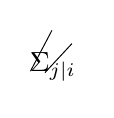
\begin{tikzpicture}[baseline=(A020G01base.base),x=0.025em,y=-0.025em]
\useasboundingbox (-2,-5) rectangle (82,85);
\node[anchor=base west,inner sep=0pt,outer sep=0pt] (A020G01base) at (1,58)
{\rlap{$\Sigma_{\unsure{j|i}}$}\phantom{$\deleted{\Sigma_{\unsure{j|i}}}$}};
\draw[line width=0.35pt] (2,58)--(33,-1);
\draw[line width=0.35pt] (23,60)--(62,18);
\end{tikzpicture}
$U_{J,i}$ est un voisinage
% A020-G02: gray detached round point, source origin (1175,817), baseline y=817.
% Shape candidate only; role, hand and surface origin unresolved. No word is in this group.
\unsure{\begin{tikzpicture}[baseline={(0,0)},x=0.025em,y=-0.025em]
\useasboundingbox (0,0) rectangle (11,24);
\fill[gray] (4,18) ellipse [x radius=2.2,y radius=2.5];
\end{tikzpicture}}
de $\deleted{\Sigma}E_{\unsure{i|j}}$, et
\[
\overline{\Sigma_i^+}\cap\deleted{\Sigma}E_i\ne\varnothing,\quad
\overline{\deleted{E}\Sigma_i^-}\cap\deleted{\Sigma}E_i\ne\varnothing.
\]
On sait donc que le nb des classes est en
% A020-G03: cancelled tout/est; fixed source origin (1457,1038), baseline y=1081.
% The observed two crossing runs replace a generic visible cancellation rule.
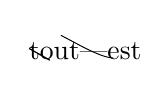
\begin{tikzpicture}[baseline=(A020G03base.base),x=0.025em,y=-0.025em]
\useasboundingbox (-2,-3) rectangle (130,53);
\node[anchor=base west,inner sep=0pt,outer sep=0pt] (A020G03base) at (0,43)
{\rlap{\unsure{tout|est}}\phantom{\deleted{\unsure{tout|est}}}};
\draw[line width=0.45pt] (0,27)--(30,44);
\draw[line width=0.35pt] (46,8)--(80,26)..controls (96,34) and (110,40)..(122,41);
\end{tikzpicture}
$(n-1)+2=n+1=\operatorname{card} I+1$ (ce qui achève \unsure{aussi|ainsi} la
% A020-G04: detached high triangular point after la; source origin (565,1395).
% Shape candidate only; role, hand and surface origin unresolved. No word is in this group.
\unsure{\begin{tikzpicture}[baseline={(0,0)},x=0.025em,y=-0.025em]
\useasboundingbox (0,-33) rectangle (12,0);
\fill (4,-31)--(7,-26)--(7,-22)--(2,-24)--cycle;
\end{tikzpicture}}
\unsure{dém.|dem.} \unsure{par|p} récurrence sur le nb des classes).

\uline{Lemme} Toute classe de $\Pi_I^\circ$ est de la forme
% A020-G05: complete formula and its added hatted label; no other words are in this group.
% Fixed source origin (1105,1660); local pixels right/down; formula baseline y=1735.
% The ordinary union operator, index, body, two parentheses and label occur once.
% The retraced left oval is drawn as the second path, beside the main brace run.
\figure{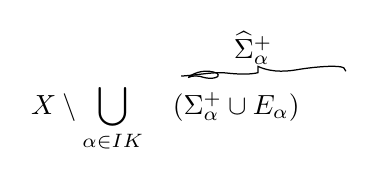
\begin{tikzpicture}[baseline=(A020G05body.base),x=0.025em,y=-0.025em]
\useasboundingbox (-210,-50) rectangle (275,145);
\node[anchor=base west,inner sep=0pt,outer sep=0pt] at (-205,75)
{$X\setminus\displaystyle\bigcup_{\alpha\in\deleted{I}K}$};
\node[anchor=base west,inner sep=0pt,outer sep=0pt] (A020G05body) at (0,75)
{$(\Sigma_\alpha^+\cup E_\alpha)$};
\node[anchor=base west,inner sep=0pt,outer sep=0pt] at (88,-6)
{$\inserted{\widehat{\Sigma}_\alpha^+}$};
\draw[line width=0.45pt] (12,20)..controls (42,18) and (60,13)..(82,16)
..controls (102,18) and (116,17)..(123,15)--(123,6)
..controls (145,16) and (168,13)..(184,10)
..controls (211,6) and (240,4)..(247,8)--(250,13);
\draw[line width=0.45pt] (22,22)..controls (33,13) and (50,10)..(64,16)
..controls (70,22) and (56,25)..(45,22)
..controls (36,19) and (29,19)..(22,22);
\end{tikzpicture}}
où $K$ est une partie
% A020-G06: complete cancelled insertion and curved guide with adjoining de I,.
% Fixed source origin (1148,1770); local pixels right/down; de I baseline y=1845.
% Exact word boundary: non vide (inserted and cancelled), de I,; partie and et remain outside.
% The phantom carries both editorial states without an extra visible generic strike.
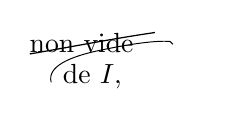
\begin{tikzpicture}[baseline=(A020G06base.base),x=0.025em,y=-0.025em]
\useasboundingbox (-3,-5) rectangle (255,94);
\node[anchor=base west,inner sep=0pt,outer sep=0pt] at (0,31)
{\rlap{\inserted{non vide}}\phantom{\inserted{\deleted{non vide}}}};
\node[anchor=base west,inner sep=0pt,outer sep=0pt] (A020G06base) at (48,75) {de $I$,};
\draw[line width=0.45pt] (0,33)..controls (59,23) and (119,11)..(181,2);
\draw[line width=0.35pt] (31,74)..controls (25,52) and (55,37)..(105,27)
..controls (143,19) and (183,13)..(203,15)--(207,19);
\end{tikzpicture}
et
% slanted
\reversemarginpar\margin{\makebox[\linewidth][r]{\rotatebox{19}{\shortstack[l]{$K$ est $\ne\varnothing$\\si $I\ne\varnothing$}}}}\normalmarginpar
$\forall\alpha\in K$, \deleted{on a} $\Sigma_\alpha^+
% A020-G07: complete observed reworked membership/arrow shape, source origin (945,1943).
% Full-state candidates: \deleted{\Rightarrow}\in | \deleted{\to}\in | \in.
% The primary is the first candidate; the third retains a live/retraced membership state.
% The phantom records the complete candidates; the local unsure qualifies the actual paths.
\mathrel{\unsure{\begin{tikzpicture}[baseline={(0,41)},x=0.025em,y=-0.025em]
\useasboundingbox (-2,-2) rectangle (55,55);
\node[overlay,anchor=base west,inner sep=0pt,outer sep=0pt] at (0,41)
{\phantom{$\deleted{\Rightarrow}\in|\deleted{\to}\in|\in$}};
\draw[line width=0.45pt] (38,4)..controls (24,1) and (1,25)..(1,33)
..controls (1,48) and (19,51)..(28,47);
\draw[line width=0.45pt] (2,33)--(41,28);
\draw[line width=0.35pt] (26,20)--(42,31)..controls (48,32) and (44,18)..(40,16);
\end{tikzpicture}}}
\pi_0(X\setminus{\unsure{E|\deleted{\Sigma}E}}_\alpha)$, tels que $\forall\alpha,\beta\in K$, $\alpha\ne\beta$, on ait $\widehat{\Sigma}_\alpha^+\cap\widehat{\Sigma}_\beta^+=\varnothing$ $(\Longleftrightarrow\Sigma_\alpha^+\cap\Sigma_\beta^+=\varnothing)$.
% archive sheet number: 19
